\documentclass{beamer}

\usepackage{enumerate}
\usepackage[utf8x]{inputenc}
%\usepackage{default}
\usepackage{hyperref}
\usepackage{graphicx,wasysym}
\usepackage{subfigure}
\usepackage{fixltx2e}%for subscript superscript
\usepackage{amsmath}
\usepackage{amsfonts}
\usepackage{setspace}
\usepackage{xcolor}
\usepackage{algorithmic}
\usepackage{caption}
%\usepackage[lined,boxed]{algorithm2e}
%\usepackage[linesnumbered,vlined,portugues]{algorithm2e} 



% latex

% Related to VCD

\newcommand{\VC}{\textrm{\sf VC}}
\newcommand{\SVC}{\textrm{\sf SVC}}
\newcommand{\negs}{\textrm{\sf negs}}
\newcommand{\VCDimC}{\textrm{\sf VCD}}
\newcommand{\SVCDimC}{\textrm{\sf SVCD}}
\newcommand{\vcd}{\textrm{{\sf VC}-dimension}}
\newcommand{\svcd}{\textrm{Subspace {\sf VC}-dimension}}

\newcommand{\Th}{\textrm{\sc Th}}

% Complexity Classes
\newcommand{\UNSAT}{\textrm{\sf UNSAT}}
\newcommand{\SAT}{\textrm{\sf SAT}}
% Fourier symbols
\newcommand{\wt}[1]{\widetilde{#1}}
\newcommand{\wh}[1]{\widehat{#1}}
\newcommand{\sse}{\subseteq}
\newcommand{\bits}{\{-1,1\}}
\newcommand{\zo}{\{0,1\}}
\newcommand{\bn}{\bits^n}
\newcommand{\zon}{\zo^n}
\newcommand{\isafunc}{:\bn\to\bits}
\newcommand{\isazofunc}{:\zo^n\to\zo}
\newcommand{\sumi}{\sum_{i=1}^n}
\newcommand{\cond}{\,|\,}
\newcommand{\defn}{\stackrel{\text{\tiny def}}{=}}
\newcommand{\zap}[1]{}
\newcommand{\ind}{\mathsf{Ind} }
\newcommand{\cpm}{C_{\oplus,\min}}
\newcommand{\degtwo}{\mathsf{deg_{\F_2}}}
\newcommand{\fhat}{\widehat{f}}
\newcommand{\ghat}{\widehat{g}}
\newcommand{\pmo}{\set{-1,1}}
\newcommand{\pmon}{\pmo^n}
\newcommand{\I}{\mathbf{I}}
\newcommand{\sps}{\mathsf{sparsity}}
\newcommand{\fdim}{\mathsf{fdim}}
\newcommand{\gr}{\mathsf{gr}}

% left-right wrappers
\newcommand{\card}[1]{\left | \set{#1}\right |}
\newcommand{\set}[1]{\left\{ #1 \right\}}
\newcommand{\cset}[1]{\left ( #1 \right )}
\newcommand{\abs}[1]{\left\lvert #1 \right\rvert}
%\newcommand{\norm}[1]{\left\lVert #1 \right\rVert}
\newcommand{\floor}[1]{\left\lfloor #1 \right\rfloor}
\newcommand{\ceil}[1]{\left\lceil #1 \right\rceil}

% latin
\newcommand{\etal}{\textit{et al}.\@\xspace}
\newcommand{\ie}{i.e.}

% models
\newcommand{\CREW}{\textsf{CREW}}
\newcommand{\DT}{\mathsf{DT}}

% Boolean function parameters
\newcommand{\sens}{\mathsf{s}}
\newcommand{\tsens}{\mathsf{ts}}
\newcommand{\bsens}{\mathsf{bs}}
\newcommand{\cert}{\mathsf{C}}
\newcommand{\altr}{\mathsf{alt}}
\newcommand{\salt}{\mathsf{salt}}
\renewcommand{\deg}{\mathsf{deg}}
\newcommand{\inv}{\mathtt{I}}
\newcommand{\indim}{\mathtt{indim}}
\newcommand{\outdim}{\mathtt{outdim}}


% short hands
\newcommand{\lep}{\preccurlyeq}
\newcommand{\pgeq}{\succcurlyeq}
\newcommand{\calA}{{\cal A}}
\newcommand{\calB}{{\cal B}}
\newcommand{\calC}{{\cal C}}
\newcommand{\calD}{{\cal D}}
\newcommand{\calE}{{\cal E}}
\newcommand{\calF}{{\cal F}}
\newcommand{\calG}{{\cal G}}
\newcommand{\calH}{{\cal H}}
\newcommand{\calI}{{\cal I}}
\newcommand{\calJ}{{\cal J}}
\newcommand{\calK}{{\cal K}}
\newcommand{\calL}{{\cal L}}
\newcommand{\calM}{{\cal M}}
\newcommand{\calN}{{\cal N}}
\newcommand{\calO}{{\cal O}}
\newcommand{\calP}{{\cal P}}
\newcommand{\calQ}{{\cal Q}}
\newcommand{\calR}{{\cal R}}
\newcommand{\calS}{{\cal S}}
\newcommand{\calT}{{\cal T}}
\newcommand{\calU}{{\cal U}}
\newcommand{\calV}{{\cal V}}
\newcommand{\calW}{{\cal W}}
\newcommand{\calX}{{\cal X}}
\newcommand{\calY}{{\cal Y}}
\newcommand{\calZ}{{\cal Z}}


% bold math : for probabiliy
\newcommand{\bldS}{\mathbf{S}}
\newcommand{\bldx}{\mathbf{x}}
\newcommand{\bldX}{\mathbf{X}}
\newcommand{\bldsbar}{\mathbf{\overline{s}}}


% Boolean functions.
\newcommand{\DISJ}{\mbox{\sf DISJ}}
\newcommand{\SDISJ}{\mbox{\sf SDISJ}}
\newcommand{\INEQ}{\mbox{\sf INEQ}}
\newcommand{\PDISJ}{\mbox{\sf PDISJ}}
%\newcommand{\AND}{\wedge}
%\newcommand{\OR}{\vee}
\newcommand{\sat}{\textrm{\bf SAT}}
\newcommand{\match}{\mbox{\sf MATCH}}
\newcommand{\MAJ}{\mathsf{MAJ}}
\newcommand{\ANDOR}{\mathop{\mbox{$\mathsf{AND}$-$\mathsf{OR}$}}}
\newcommand{\ADDR}{\mathsf{ADDR}}

% math symbols
\newcommand{\expct}[1]{\mathbb{E}\left[ #1 \right]}
\newcommand{\gaussian}[3]{ {#1 \brack #2}_{#3}}

% communication complexity
\newcommand{\CC}{\mathsf{CC}}


% fields
\newcommand{\field}{\mathbb{F}}
\newcommand{\F}{{\mathbb{F}}}
\newcommand{\Q}{{\mathbb{Q}}}
\newcommand{\N}{{\mathbb{N}}}
\newcommand{\R}{{\mathbb{R}}}

% linear algebra
\newcommand{\rank}[1]{\mathsf{rank} \left( #1 \right)}
\newcommand{\rspace}[1]{\mathsf{rowspace} \left( #1 \right)}
%\newcommand{\degtwo}{\mathsf{deg_{\F_2}}}
\renewcommand{\deg}{\mathsf{deg}}


\usetheme{Boadilla} % Taken from Overleaf
\graphicspath{ {./images/} }

%\usetheme{Berlin} %writes content horizontally on top
%\setbeamertemplate{page number in head/foot}[totalframenumber] %gives slide number





\setbeamercolor{title}{fg=red!40!black}
%\setbeamercolor{title}{fg=red!40!black,bg=green!40!white}

\title{ \sc \color{blue}{Optimal Bounds for Open Addressing Without Reordering}}
\subtitle{Martin Farach-Colton , Andrew Krapivin , William Kuszmaul}
\author{Presented by - Amit Roy }
\institute{}
% NUS - \date{August 21,  2023}
\date{March 27, 2025}



\begin{document}
 
\begin{frame}
\titlepage
\end{frame} 



\section{Introduction}

\begin{frame}{Hash Table}
	\begin{itemize}
		\item Support dictionary operations - {\sc Insert, search} and {\sc delete} 
		\item Uses a hash function $h:[u]\to [m]$ to index keys
	\end{itemize}

\begin{figure}
	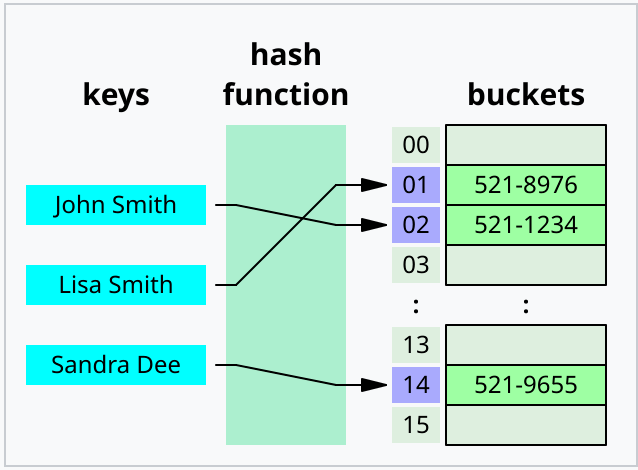
\includegraphics[scale=0.5]{images/hashing.png}
\end{figure}

%\footnote{Image Credit: Wikipedia}

\end{frame}
\begin{frame}
	{\bf Collision Resolutions}
	\begin{itemize}
		\item Chaining - Each slot in the table is a pointer to a linked list which stores the keys
		\item Open Addressing - All elements occupy the hash table itself
%		\begin{itemize}
%			\item Linear Probing - $h(k,i) = (h_1(k) + i) mod m$
%			\item Quadratic Probing - 
%			\item Double Hashing - $h(k,i) = (h_1(k) + ih_2(k)) mod m$
%		\end{itemize}
	\end{itemize}
\end{frame}

\begin{frame}{Chaining vs Open-Addressing}
	\centering
	\begin{minipage}{0.48\textwidth}
		\centering
		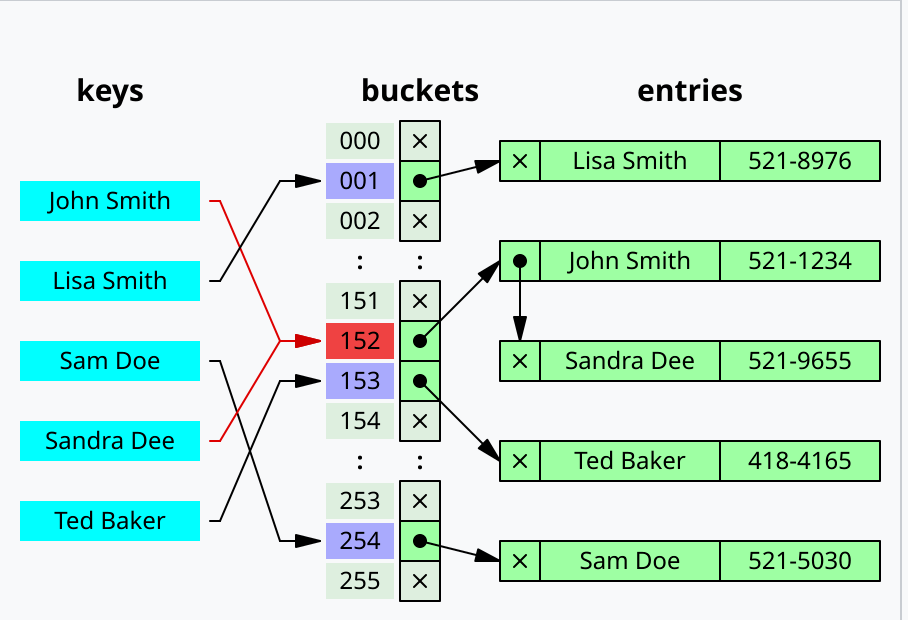
\includegraphics[width=\linewidth]{chaining.png}
		\captionof{figure}{Chaining}
	\end{minipage}
	\hfill
	\begin{minipage}{0.48\textwidth}
		\centering
		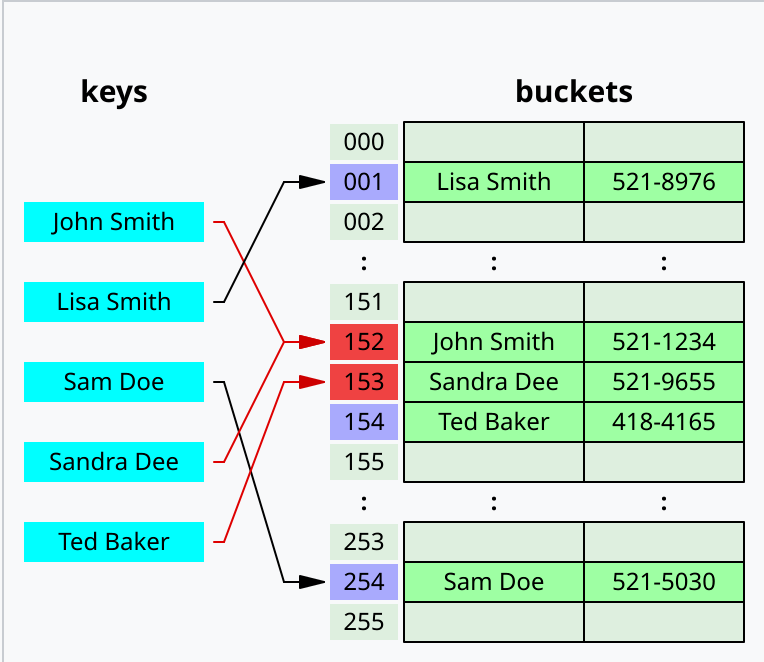
\includegraphics[width=\linewidth]{open-addressing.png}
		\captionof{figure}{Open Addressing}
	\end{minipage}
\footnote{Image Credit : Wikipedia}

\end{frame}

\begin{frame} {Definitions}
	\begin{block}{Probe Complexity}
		\begin{itemize}
			\item The number of probes that an algorithm has to make to insert/search the key is called the probe complexity of the key.
			\item For example, for a key $k$, if an algorithm probes $h_1(k), h_2(k), \ldots, h_t(k)$ to find an empty slot to insert the key, then the probe complexity of $k$ is $t$.
		\end{itemize}
	\end{block}

\begin{block}{Uniform Probing}
	For a given key $k$, the probe sequence - $h_1(k), h_2(k), \ldots, h_t(k)$ is a random permutation of $\set{1, 2, \ldots,n }$
\end{block}
\end{frame}


\begin{frame}{Greedy and Non-greedy Open-Addressing}
	\begin{itemize}
		\item {\bf Greedy :}  Any algorithm in which each element uses the first unoccupied position in its probe sequence.
		\item {\bf Non-greedy :} May probe further before inserting the element in the hash table
	\end{itemize}	
\end{frame}

\begin{frame}{Previous Work}
	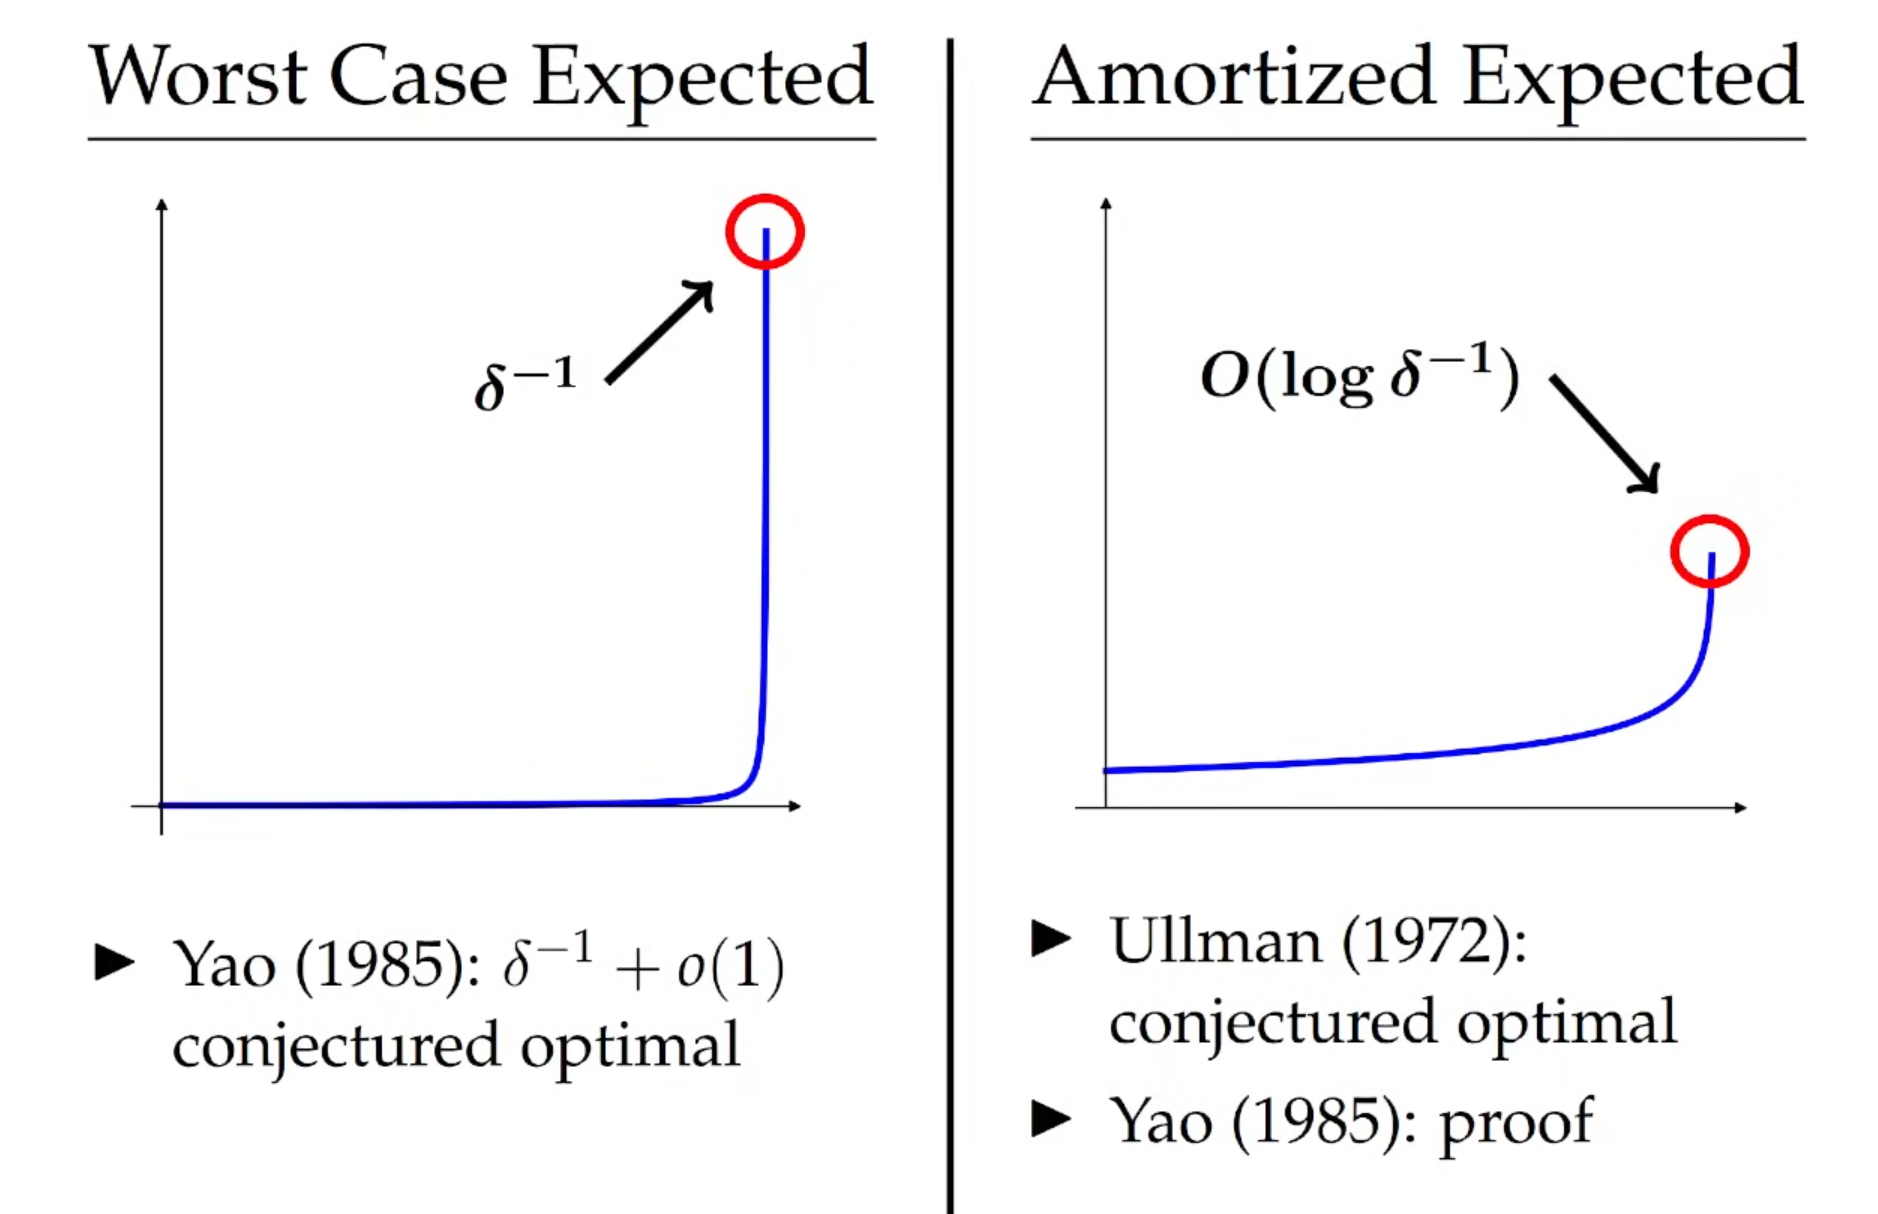
\includegraphics[scale=0.35]{previous-work}
\end{frame}

\begin{frame}{Results}
	
	\begin{enumerate}
		\item Greedy
		\begin{itemize}
			\item Amortized expected probe complexity - $\calO(\log{\delta^{-1}})$
			\item Worst-case expected probe complexity $\calO(\log^2{\delta^{-1}})$
			\begin{itemize}
				\item \alert{Yao's conjecture of bound $\theta(\delta^{-1})$ proven false.}
			\end{itemize} 
			\item High-probability worst-case probe complexity $\calO(\log^2{\delta^{-1}} + \log{\log{n}})$
			\begin{itemize}
				\item Matching lower bound
			\end{itemize}
		\end{itemize}
	\vspace{10mm}
	\item Non-Greedy 
	\begin{itemize}
		\item Amortized probe complexity $\calO(1)$
		\item Worst-case expected probe complexity $\calO(\log{\delta^{-1}})$ %(\alert{prev $\calO()$})
		\begin{itemize}
			\item Matching lower bound
		\end{itemize}
	\end{itemize}
	\end{enumerate}
\end{frame}


\begin{frame}
	\begin{block}{Theorem - Greedy Open-Addressing}
		Let $n \in \mathbb{N}$ and $\delta \in(0, 1)$ be parameters such that $\delta > 
		\calO(1/n^{o(1)})$.
			 There exists a { \bf greedy} open-addressing strategy that supports $n - \floor{\delta n}$ insertions that has 
			\begin{itemize}
				\item worst-case expected probe complexity (and insertion time) - $\calO(\log^2{\delta^{-1}} )$ 
				\item worst-case probe complexity over all insertions - $\calO(\log^2{\delta^{-1}} + \log{\log{n}})$, with prob $1- 1/poly(n)$, 
				\item amortized expected probe complexity - $\calO(\log{\delta^{-1}})$
			\end{itemize}
		
	\end{block}
\end{frame}

\begin{frame}{Funnel Hashing}
	\begin{figure}
		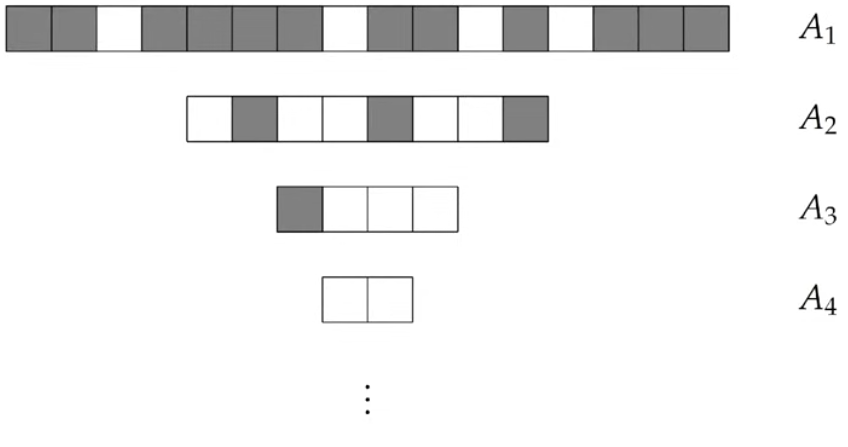
\includegraphics[scale=0.5]{funnel_hash.png}
	\end{figure}
\end{frame}

\begin{frame}{Funnel Hashing}
	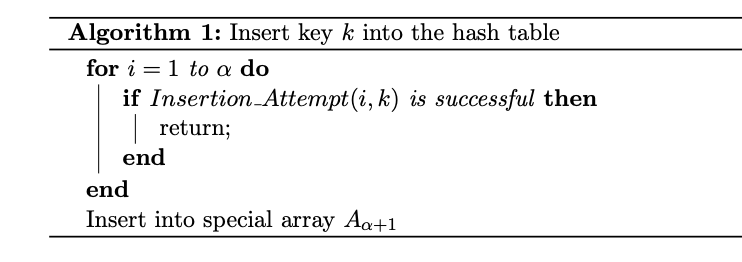
\includegraphics{insert}
\end{frame}

\begin{frame}{Funnel Hashing}
	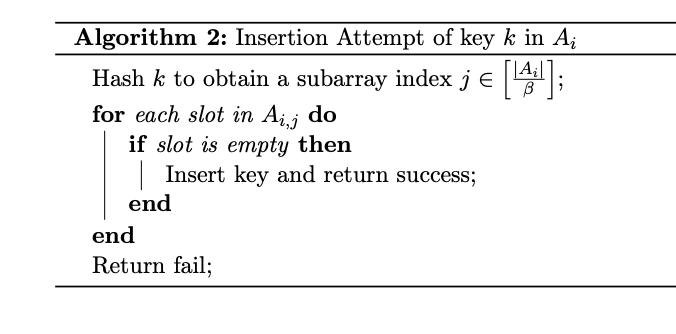
\includegraphics{insertion-attempt}
\end{frame}

\begin{frame}{Analysis}
	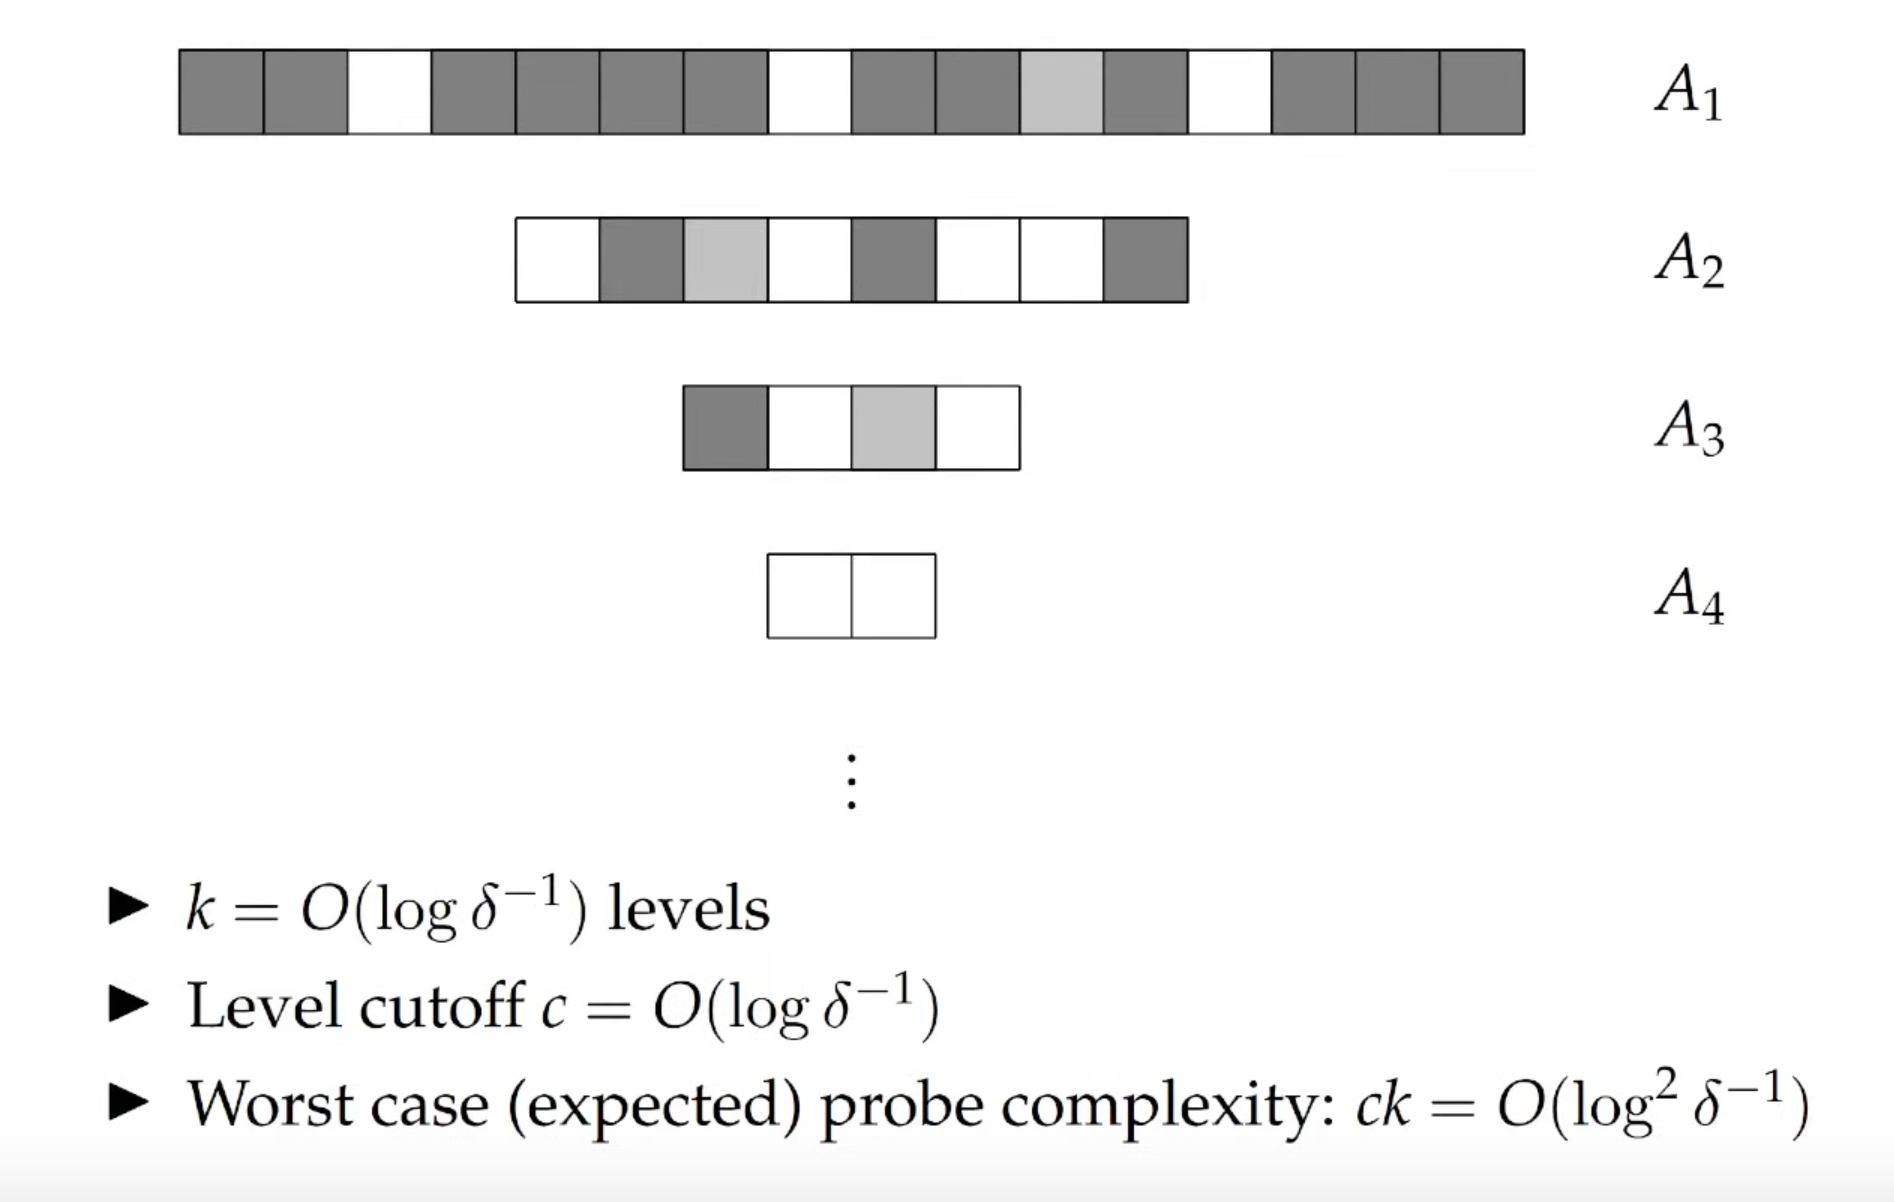
\includegraphics[scale=0.3]{analysis}
\end{frame}


\begin{frame}{Algorithm for special array $A_{\alpha + 1}$}
	\begin{enumerate}
		\item Split $A_{\alpha + 1}$ into two subarrays $B$ and $C$ of equal size. 
		\item First, try to insert in $B$. Upon failure insert into $C$ ( insertion to $C$ is guaranteed to succeed with high probability)
		\item $B$ is implemented as a uniform probing table, and we give up searching through $B$ after $\log{\log{n}}$ attempts.
		\item $C$ is implemented as a two-choice table with buckets of size $2\log{\log{n}}$. 
	\end{enumerate}
	
\end{frame}

\begin{frame}{Proof}
	\begin{block}{Lemma 1}
		For a given $i \in \alpha$, we have with probability $1 - \frac{1}{n^{\omega(1)}}$ that, after $2|A_i|$ insertion attempts have been made in $A_i$, fewer than $\frac{\delta}{64} |A_i|$ slots in $A_i$ remain unfilled.
	\end{block}

	\begin{block}{Lemma 2}
		The number of keys inserted into $A_{\alpha + 1}$ is fewer than $\frac{\delta}{8}n$, with probability $1 - \frac{1}{n^{\omega(1)}}$.
	\end{block}

\end{frame}






\begin{frame}{Probe Complexity of $A_{\alpha + 1}$}
	Complexity of inserting into $B$ - 
	\begin{enumerate}
		\item $B$ has size $A_{\alpha + 1}/2 \ge \delta n/4$, so load factor never exceeds $1/2$. 
		\item Each insertion makes $\log{\log{n}}$, each of which has success probability of $1/2$. 
		\item Thus, expected number of probles is $\calO(1)$
		\item Probability that insertion fails after all attempts is $1/2^{\log{\log{n}}} \le 1/ \log{n}$.
	\end{enumerate}
\end{frame}

\begin{frame}{Proof - Insertion into $C$ of $A_{\alpha+1}$}
	\begin{block}{Lemma: Power of two choices}
		If $m$ balls are placed into $n$ bins by choosing two bins uniformly at random for each ball and placing the ball into the emptier of the two bins, then the maximum load of any bin is $m/n + \log{\log{n}} + \calO(1)$ with high probability in $n$.
	\end{block}
\end{frame}

\begin{frame}{Probe Complexity of $A_{\alpha + 1}$}
	Complexity of inserting into $C$ - 
	\begin{enumerate}
		\item Recall, $C$ is implemented as a two choice table with buckets of size $2\log{\log{n}}$
		\item From Lemma we have that, with high probability, no bucket in $C$ overflows. 
		\item Expected time of each insertion in $C$ is at most $o(1)$.
	\end{enumerate}
\end{frame}

\begin{frame}{Analysis}
	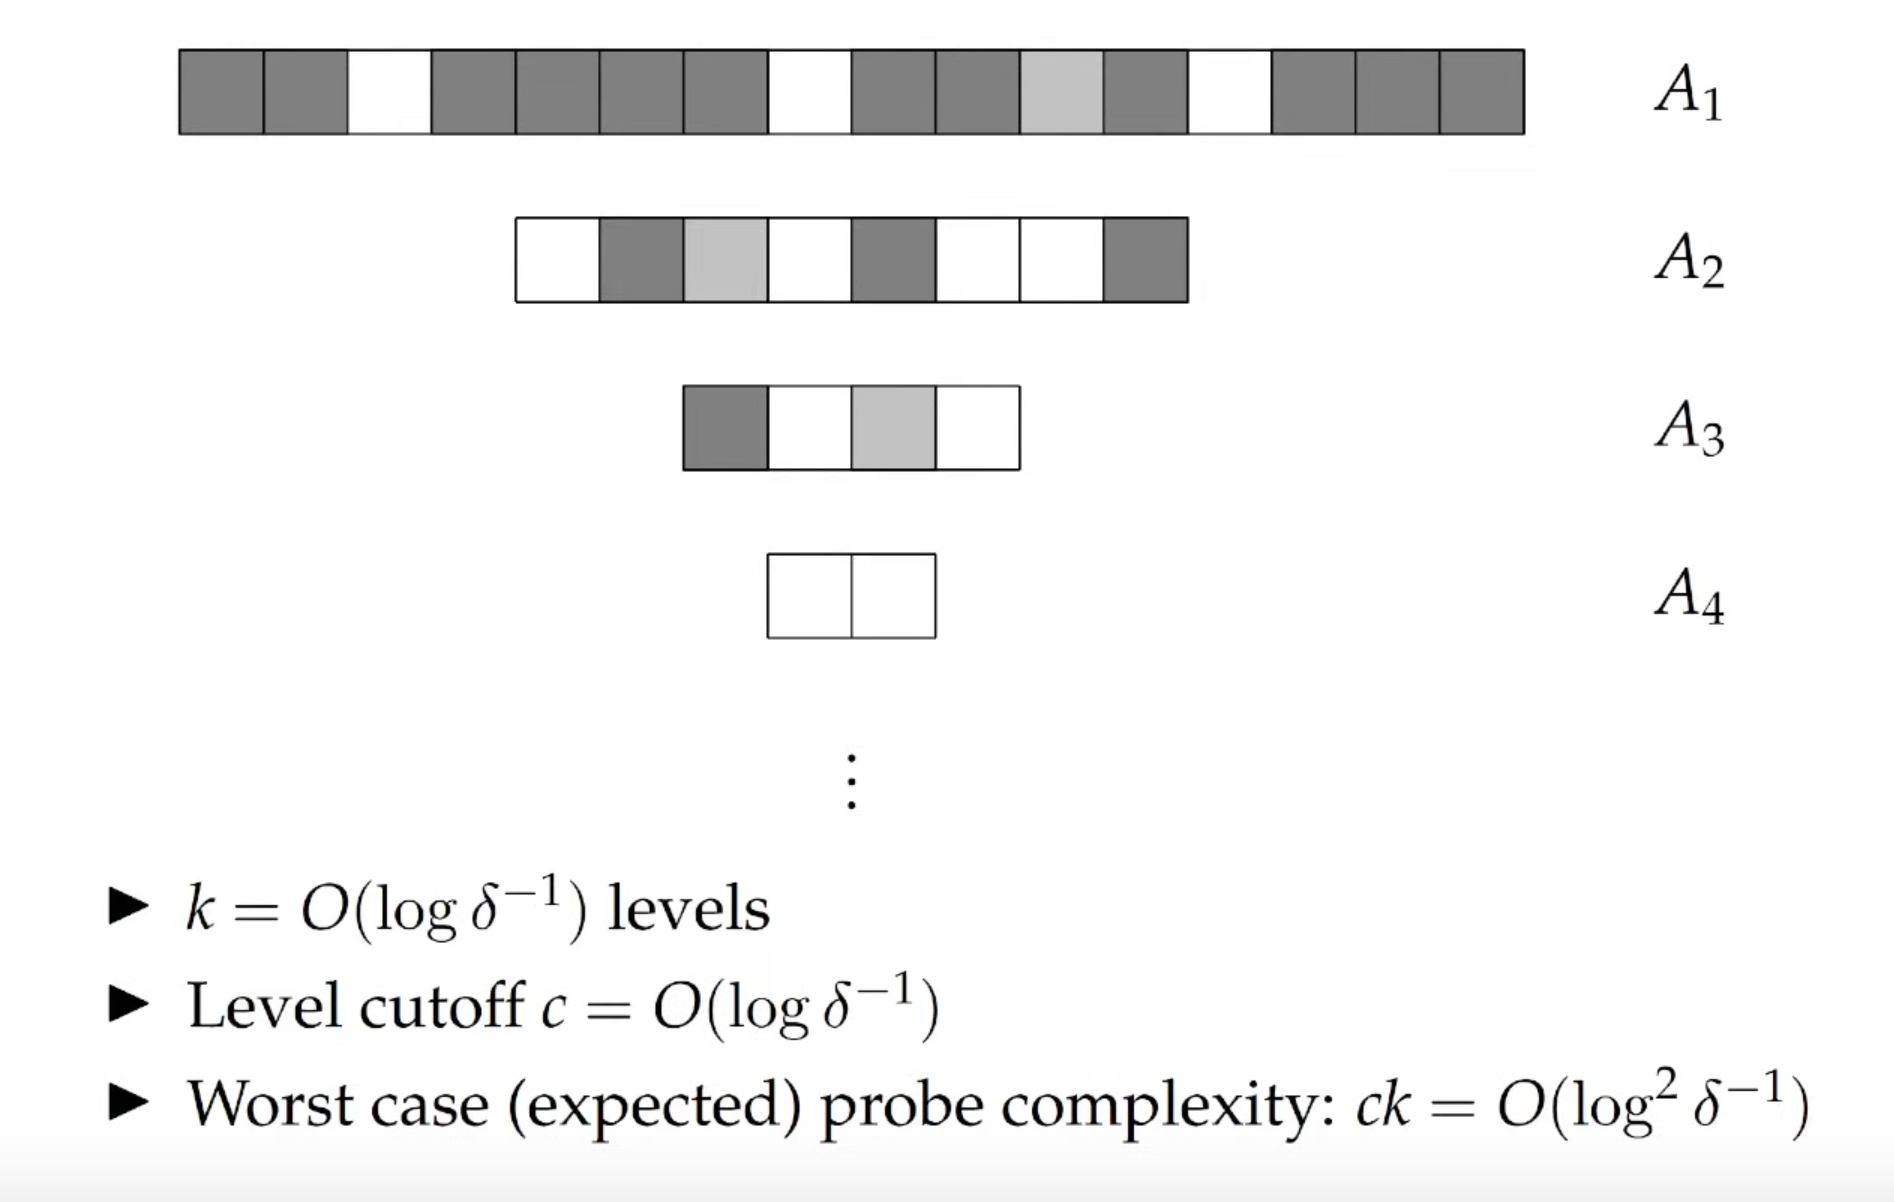
\includegraphics[scale=0.3]{analysis}
\end{frame}

\begin{frame}{Proof}
	\begin{itemize}
		\item Total $\alpha$ arrays , and cutoff probes $\beta$ in each $A_i$ 
		\item Probe complexity of each insertion - $\beta\alpha + f(A_{\alpha + 1})$ 
		\item Assume $\delta \le \frac{1}{8}$. Let $\alpha = \lceil 4\log{\delta^{-1} + 10} \rceil$ and $\beta = \lceil 2\log{\delta^{-1}}\rceil$
		\item Probe Complexity - $\calO(\log^2{\delta^{-1}}) + f(A_{\alpha+1})$ 
		\item  Hence, $\calO(\log^2{\delta^{-1}})$ in worst-case expected probe  complexity and a high-probability worst-case probe complexity of $\calO(\log^2{\delta^{-1}} + \log{\log{n}})$.
	\end{itemize}
\end{frame}


\begin{frame} {Other Results}
	1. {\bf Elastic Hashing}
	\begin{block}{Theorem - Non-greedy Open-Addressing}
		Let $n \in \mathbb{N}$ and $\delta \in(0, 1)$ be parameters such that $\delta > 
		\calO(1/n)$. There exists an open-addressing hash table that supports $n - \floor{\delta n}$ insertions in an array of size $n$, that does not reorder items after they are inserted, and that offers -
		\begin{itemize}
			\item amortized expected probe complexity $O(1)$
			\item worst-case expected probe complexity $\calO(log \delta^{-1})$, and
			\item worst-case expected
			insertion time $\calO(log \delta^{-1})$.
		\end{itemize}
	\end{block}
\end{frame}


\begin{frame}{Other Results}
	2. {\bf Lower Bounds}
	\begin{block}{Theorem - Lower Bound for Greedy Algorithms}
			Let $n \in \mathbb{N}$ and $\delta \in(0, 1)$ be parameters such that $\delta$ is an inverse power of two. Consider any greedy open-addressed hash table with capacity $n$. If $(1-\delta)n$ elements are inserted into the hash table, then the final insertion must take expected time $\Omega(\log^2{\delta^{-1}})$.
	\end{block}
\end{frame}

\begin{frame}{More Proofs}
	\begin{block}{Lemma 2}
		The number of keys inserted into $A_{\alpha + 1}$ is fewer than $\frac{\delta}{8}n$, with probability $1 - \frac{1}{n^{\omega(1)}}$.
	\end{block}
\begin{itemize}
	\item From {\bf Lemma 1}, every {\em fully-explored} $A_i$ is at least $(1-\delta / 64)$ full, where {\em fully-explored} means at least $2|A_i|$ insertion attempts made to $A_i$.
	\item Let $\lambda \in [\alpha]$ be largest index s.t. $A_{\lambda}$ receives fewer than $2|A_{\lambda}|$ insertion attempts. 
	\item {\bf Case 1: $\lambda \le \alpha - 10$} 
	\begin{itemize}
		\item For $i>\lambda$, $A_i$ contains at least $|A_i|(1-\delta/64)$ keys. 
		\item Total keys in $i \ge \lambda$ : $(1-\delta/64) \sum_{i=\lambda+1}^{\alpha}|A_i| \ge 2.5(1-\delta/64)|A_{\lambda}|$
		\item This contradicts that $A_{\lambda}$ received at most $2|A_{\lambda}|$ insertion attempts.
	\end{itemize}  
\end{itemize}
\end{frame}

\begin{frame}{Lemma 2 Proof Contd}
	\begin{itemize}
		\item {\bf Case 2 : $\alpha -10 < \lambda \le \alpha$} 
		\begin{itemize}
			\item Fewer than $A_{\alpha -10} < n \delta/8$ keys are attempted to be inserted in $A_i$ with $i\ge \lambda$. Hence, we are good.
		\end{itemize}
	\item {\bf Case 3: $\lambda = null$} 
	\begin{itemize}
		\item Each $A_i$ has at most $\delta |A_i|/64$ empty slots.
		\item Total empty slots at the end of insertion : $|A_{\alpha+1}| + \sum_{1}^{\alpha}\frac{\delta|A_i|}{64} < n\delta$
		\item This contradicts that after $n(1-\delta)$ insertions, there are at least $n\delta$ slots empty.
	\end{itemize}
	\end{itemize}
\end{frame}

\begin{frame}{Proof of Lemma 1}
		\begin{block}{Lemma 1}
		For a given $i \in \alpha$, we have with probability $1 - \frac{1}{n^{\omega(1)}}$ that, after $2|A_i|$ insertion attempts have been made in $A_i$, fewer than $\frac{\delta}{64} |A_i|$ slots in $A_i$ remain unfilled.
	\end{block}

\end{frame}

\begin{frame}
\begin{center}
{\sc \LARGE Thoughts and Questions ?} \\
\vspace{3cm}
{\sc \large Thanks} 
\end{center}
\end{frame}


%%Bibliography

\bibliographystyle{alpha}
%\bibliography{VCbib}

\end{document}